\section{Object Dectection Based on Combination of Multiple Features}
\label{sec:objectdetection}
In the first stage, we try to detect object by combination many
features including both global and local features. Up to present, we
have tested with seven features, such as: edge, corner, HoG, line,
circle, SURF, and color. This section describes how to extract and use
these features for recognize object.
\subsection{Edge, Corner and HoG Feature}
It is easy to see that the most important features for recognition
object are the overall shape of that object and all boundaries which
separate main parts of object. Shape or boundary is basically
composed by edges. These edges are arranged in a specific order and
meet each other at some points called corners. Beside, edge
orientation also plays a prominent role for figuring object. With the
same number of edges, but in different order and different orientation,
it makes viewer imagine different objects. The description of how
these principal components make object imaginable is in Fig.~\ref{fig:3components}.
\begin{figure}[ht]
  \centering
  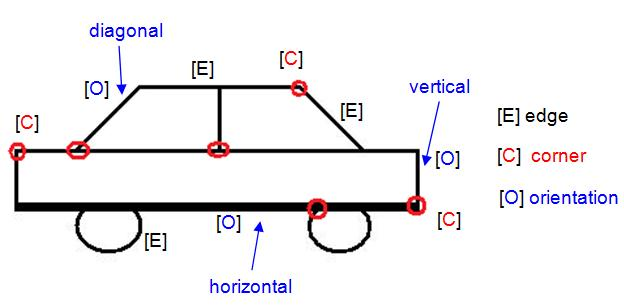
\includegraphics[width=2.20in]{images/edge_cornre_HoG.jpg}
  \caption{Three main components make object be figured.}
  \label{fig:3components}
\end{figure}

Based on this, we propose an overall approach for object detecting
which focuses on edge, corner and edge orientation (HoG). More
detail is presented in the next diagram in Fig~\ref{fig:framework}. But there is still an
issue in this model. That is how do we know that edge/corner is at
right position or not? In order to answer this question, we must point
out the place where edge/corner must belong to before detecting
object. Actually, there are many way to specify location of
edge/corner, such as using prior knowledge, or machine learning, etc.
\begin{figure}[ht]
  \centering
  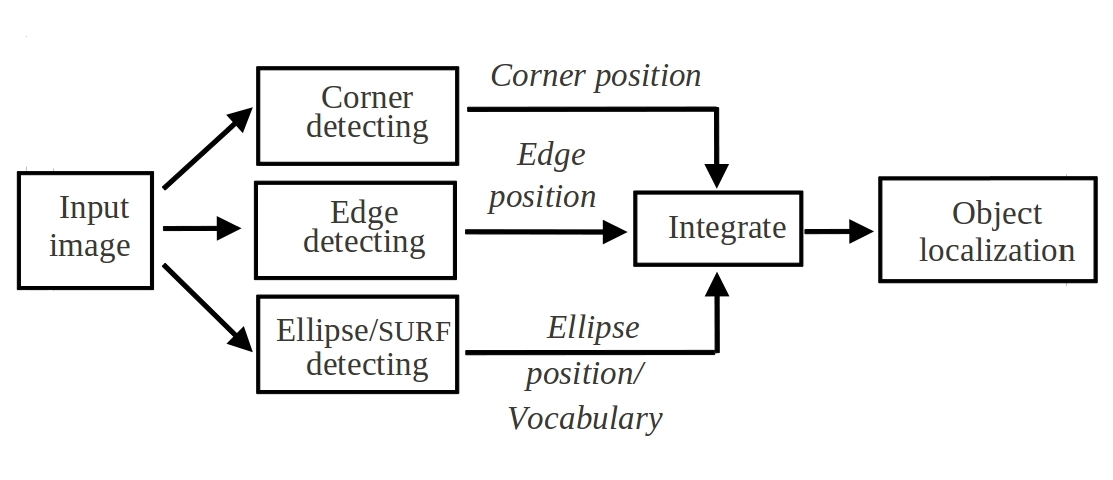
\includegraphics[width=3.15in]{images/framework1.jpg}
  \caption{Object detection based on multiple features.}
  \label{fig:framework}
\end{figure}
In our implement, we choose machine learning approach because
it is more general for a lot of objects and one most
important reason is that it requires no user's prior knowledge about object that they want to detect.

\textit{Edge and corner detection }
Up to present, there are a lot of implementations of edge/corner
detection and get the result with a high accuracy rate. Many of them
have been reported in public. Zuniga and Haralick fit a continuous
surface over a small neighborhood of each point and consider the
rate of change in gradient direction. Moravec defined 'points of interest' as points where there is a 
large intensity variation in every direction. Harris and Stephens used image derivatives to estimate the
autocorrelation of the image. Rangarajan, Shah and Brackle found an
optimal function representing the corner detector which when
convolved with the gray level function yields a maximum at the
corner point. Rafajlowicz, E. uses the idea of vertically weighted
regression and in its simplest form it leads to interpreting SUSAN in
terms of a box sliding on the surface of an image. This modification
of the SUSAN algorithm is still simple, robust against errors and
provides thinner edges, without further efforts on additional thinning.
Canny introduces the notion of non-maximum suppression, which
means that given the pre-smoothing filters, edge points are defined
as points where the gradient magnitude assumes a local maximum in
the gradient direction. Sonya Coleman et al~\cite{coleman2007integrated}
proposed a new method for enabling edge and corner detection to be
integrated with a significantly reduced computation time.
In our performance, we have tried with many methods for
edge/corner detecting, and Canny detector gave the
best result for edge detection, while Harris detector worked well with
corner detection.

\textit{Edge orientation detection }
Specifying orientation of each edge is not an easy task. Because,
with all edge detection method above, we only get the total edge
image not each separate edge in image. So, it is almost impossible to
know the orientation of each edge due to we don t specify each edge
individually. Instead of that, we can calculate the domain orientation
of all edge in a specific sub-image. From this, we can define
relatively the edge orientation. The domain orientation of a region
can be calculated with HOG descriptor method (Histogram of
Oriented Gradient). HOG descriptor is a local statistic of the
orientations of the image gradients around a keypoint. HOG
descriptor was initially proposed by Lowe in his Scale Invariant
Feature Transform (SIFT)~\cite{lowe2004distintive}. Several HOG-based algorithms have
been recently presented~\cite{bay2008surf} and combined with technologies such as
boosted classifiers~\cite{dalal2005histograms}, in which Navneet Dalal and Bill Triggs (INRIA) have
used this method for human detection with a high accuracy rate.
David Monzo et al~\cite{monzo2008hog} compared HOG-EBGM vs. Gabor-EBGM
and showed the result that HOG had a better performance.

\textit{Making edge map and corner map }
\textit{Edge map/corner map} is used to know if edge/corner is at right
position or not. To make edge map and corner map, we use the same
method as Zhenfeng Zhu et al~\cite{zhu2004car}. For all images in the positive
training-image set ($T_{pos}$) (the rest of training-image set is negative,
$T_{neg}$), after detecting edge/corner we accumulate them in one temp
image $T_{e}$ or $T_{c}$. Then edge map and corner map will be made from
these temp images respectively. However,~\cite{zhu2004car} makes edge map and
corner map be binary images. Our performance shows that with gray
scale image, the result will be better. With a binary map, the location
of edge or corner must be fixed at that position. But, due to variant
of scale or view point, the location of edge or corner cannot be fixed
at one specific point, other while it can be swung in a small region.
Intuitively, gray scale map works better in this case.
\begin{figure}[ht]
  \centering
  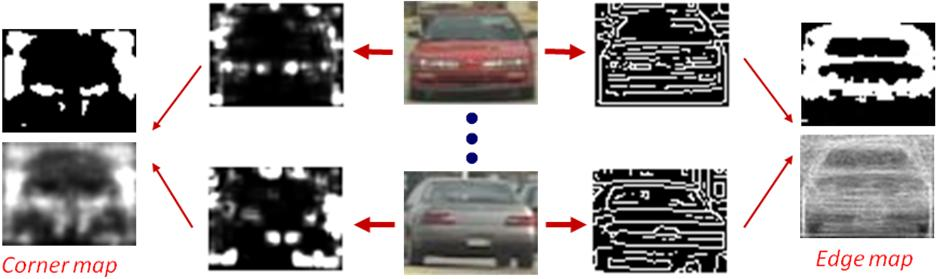
\includegraphics[width=3.25in]{images/edgemap_cornermap.jpg}
  \caption{Making Edge map and Corner map from training set.}
  \label{fig:making_edge_corner_map}
\end{figure}
The edge map $M_{E}(x,y)$ and corner map $M_{C}(x,y)$ are constructed from
$T_{e}$ and $T_{c}$ as following
\begin{equation}
M_E(x,y) = \frac{T_{e}(x,y)}{\theta_1 \times N} \mbox{~~~~and~~~~}
M_C(x,y) = \frac{T_{c}(x,y)}{\theta_2 \times N}
   \label{eq:edge_corner_map}
\end{equation}
where $N$ is the number of images in the training set; $\theta_1, \theta_2$ are
specific thresholds. %hreshold $\theta_1$ equals to 25 and value 35 is for $\theta_2$. 
\subsection{SURF Feature}
In order to increase the accuracy rate, after a candidate satisfies edge
map, corner map and orientation of edge, that candidate is continuously
passed to SURF~\cite{bay2008surf} checking stage. We choose SURF because it
is invariant with scale, illumination, and similar but faster than SIFT.
\begin{figure}[ht]
  \centering
  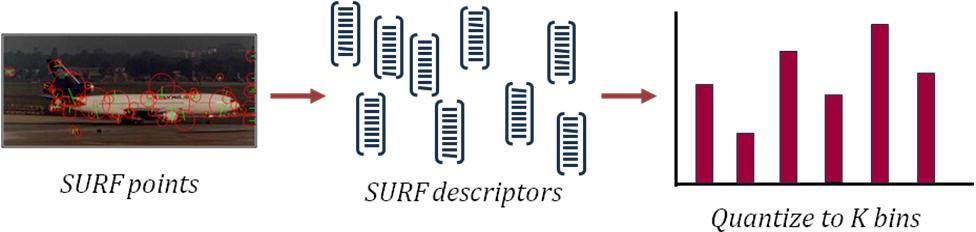
\includegraphics[width=3.25in]{images/surf.jpg}
  \caption{Making vocabulary for matching SURF feature.}
  \label{fig:making_surf}
\end{figure}
Method of matching between two set of SURF descriptors as
Gabriella et al in\cite{lazebnik2006beyond,csurka2004visual} is used. Bag of keypoints or vocabulary
are made by quantizing all descriptors from training image set to K
bins. Once descriptors have been assigned to form feature vectors,
we use Naïve Bayes classifier to determine whether an input image
belongs to one category or not by taking the largest posterior score,
$argmax\{P(C_j|I)\}$
\begin{equation}
   P(C_j|I) \propto P(C_j)P(I|C_j)= P(C_j)\prod_{t=1}^{k} N^{(t,I)} P(v_t|C_j)
   \label{eq:surf}
\end{equation}
where $I$ is new image, $C_j$ is category class (object/non-object), $v_t$
represents for keypoint or cluster center, and $N^{(t,I)}$ is the number of
times that keypoint $v_t$ occurs in image $I$.
\subsection{Color Feature}
With some objects such as horse, sheep,
their color changes not much. Color is then
a good point to distinguish object and non-
object. We mark which color belongs to
object by making color map from training
images after converting to HSV space.
Follow is an example of horse color map
from all HSV images. Inside the yellow
boundary is horse-color region, other
while outside is non-horse color region.
Color matching is calculated by
\begin{figure}[ht]
  \centering
  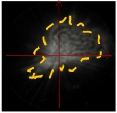
\includegraphics[width=0.90in]{images/colormap.jpg}
  \caption{Horse color map.}
  \label{fig:horse_color}
\end{figure}
\begin{equation}
   M_{color} = \sum_{x,y} CM(x,y) * H(x,y)
   \label{eq:color}
\end{equation}
which $CM$ is color map and $H$ is histogram of image in $HSV$ space.
After extract feature, in order to determine feature is used for
detecting a specific object or not, we should know if that feature
satisfies object. Value of feature $f$ in an image $i$ is written as $val(f,i)$.

\textit{Definition 1:} With a given image $i$, one feature $f$ is called satisfy ,
written as $sat(f,i)$, if the value of feature $f$ in image $i$ falls into the range of all
values of $f$ in the set of positive images - $T_{pos}$
\begin{equation}
   {argmin}(val(f,i_{pos}) \leq val(f,i) \leq {argmax} (val(f,i_{pos})
   \label{eq:sat_f}
\end{equation}
with all images $i_{pos} \in T_{pos}$

\textit{Definition 2:} A given image $i$ is called satisfy a feature set $F$,
written as $sat(F,i)$, if the image $i$ satisfies all features $f$ of $F$
\begin{equation}
   sat(F,i): \forall f \in F, sat(f,i) = True
   \label{eq:sat_F}
\end{equation}
\textit{Definition 3:} With a given image set $I$, and a feature set $F$, a subset of $I$ satisfying $F$ is called $sat(F,I)$ 
\begin{equation}
   sat(F,I) = \{i \in I, sat(F,i)\}
   \label{eq:sat_F_I}
\end{equation}
We only describe Edge, Corner, HoG, SURF and Color feature.
With Circle feature, Line feature we use Hough Transform to extract. In the next section, an algorithm for automatically determining which feature to be good to recognize a given object is presented.





